\PassOptionsToPackage{sols}{handout}
\documentclass[main]{subfiles}
\setcounterrefbeforedot{chapter}{m-ws3-2}
\setcounterrefafterdot{section}{m-ws3-2}
\addtocounter{section}{-1}
\usepackage{solutions}

\begin{document}

\ifSubfilesClassLoaded{%
  \chaptermark{\chapterthree}
}{}

\section{Applications of Trig Derivatives} \label{ws3-2}

\begin{problemonly}
    \begin{framed}

\textbf{Key Idea}:

\begin{itemize}[topsep=0pt,partopsep=0pt,parsep=8pt,itemsep=0pt]

\item You should be comfortable using trigonometric functions
and their derivatives to solve a variety of problems, including
  related rates, curve sketching, and optimization problems.

\end{itemize}
\end{framed}
\end{problemonly}


\note{One thing to look out for on some of these problems is that
  students' pictures may be oriented in all different directions. You can
  either start the problems and draw the pictures together, or you can
  just be on the lookout for when a student's picture is merely different
  from others and when it's inaccurate. A good check is whether the sign
  of the answer is appropriate.

  It may also be useful to review problem solving strategies. The
  strategies for optimization and related rates are slightly different,
  but there are some commonalities:
  \begin{enumerate}
  \item Draw a picture and label variables and constants. If it helps,
    draw two different pictures, one generic and one snapshot.
  \item Identify your goal in mathematical terms.
  \item Write an equation relating the different variables.
  \item Use differentiation to answer the question.
  \item Check that you've answered the question and that your answer is
    reasonable and within the domain.
  \end{enumerate}
}

\begin{enumerate}

\item
\begin{problem}[\stretch{0.4}]
  In our last class, in order to unpack the expression $\sin(x+h)$
  we used the addition formula $\sin(A+B)=\sin A \cos B + \sin B \cos A$.
  Use this to find an expression for $\sin(2A)$.

  Verify that this double angle formula works in the case where
  $A=\frac{\pi}{6}$.
\end{problem}

\begin{solution}
Let $B=A$. Then $\sin(A+A)=\sin A \cos A  + \sin A \cos A = 2\sin A \cos A$.
When $A=\frac{\pi}{6}$, then $\sin(2A)=\sin\frac{\pi}{3}=\frac{\sqrt3}{2}$. Using our double angle formula, $\sin(2A)=2\sin\frac{\pi}{6}\cos\frac{\pi}{6}=
2(\frac{1}{2})(\frac{\sqrt3}{2})=\frac{\sqrt3}{2}$.
\end{solution}

\item 
\begin{problem}
You are flying a kite that is 50 feet above the ground. It is moving away from you horizontally at a speed of 10\,ft/s. How fast is the angle between the string and the horizontal changing when you have let out 100 feet of string?
\end{problem}
\pspace{\vfill}

\begin{solution}

\ideas{Let's start by drawing two pictures, a generic
        picture that applies at any time, and a ``snapshot'' showing the
        situation at the time we care about.  We'll also label some
        variables in the generic picture.} 

\begin{tabular}{ccc}
Generic && Snapshot \\
\begin{tikzpicture}[scale=0.5]
    \coordinate (O) at (0,0);
    \node[circle,fill, inner sep=1.5pt] at (O) {};
    \coordinate (K) at (2,5);
    \draw[very thick] (-2,0) -- (4,0);
    \draw[thick] (O) -- (K);
    \draw (0.5,0) arc(0:68.2:0.5);
    \node at (0.7,0.5) {$\theta$};
    \draw[dashed] (K) -- node[midway, right] {$50$ ft}(O-|K);
    \node[draw=black,thick,fill=white, shape=diamond,inner sep=3pt] at (K) {};
    \node[below] at (1,0) {$x$};
\end{tikzpicture}&&
\begin{tikzpicture}[scale=0.5]
    \coordinate (O) at (0,0);
    \node[circle,fill, inner sep=1.5pt] at (O) {};
    \coordinate (K) at (8.6,5);
    \draw[very thick] (-2,0) -- (10,0);
    \draw[thick] (O) -- node[midway, above left] {$100$ ft} (K);
    \draw (0.5,0) arc(0:30:0.5);
    \node at (1.5,0.4) {$\pi/6$};
    \draw[dashed] (K) -- node[midway, right] {$50$ ft}(O-|K);
    \node[draw=black,thick,fill=white, shape=diamond,inner sep=3pt] at (K) {};
    \node[below] at (4.3,0) {$50\sqrt3$ ft};
\end{tikzpicture}
\end{tabular}

\ideas{Next, we figure out what we know and what we want to know.}

      \highlight{
        \textbf{What we know:} $\diff{x}{t} = 10$ (positive
        because $x$ is increasing)

        \textbf{What we want to know:} $\diff{\theta}{t}$
      }

      \ideas{Now, we relate the variables.  In this case, since the
        rate we know is $\diff{x}{t}$ and the rate we want to
        know is $\diff{\theta}{t}$, we need to relate $x$ and $\theta$.}

      \highlight{\textbf{Equation relating our variables:} $\tan \theta =
        \dfrac{50}{x}$} 

      \ideas{Once we have our relationship, we differentiate both sides
        with respect to $t$.}
      \begin{align*}
        \diff*{\tan \theta}{t} &= \diff*{\left[
          \frac{50}{x} \right]}{t} \nonumber \\
        \sec^2( \theta) \diff{\theta}{t} &= -\dfrac{50}{x^2}
        \diff{x}{t}
 \\
        \intertext{Plug in the snapshot information. Note: even if we didn't know that the angle at this instant was $\pi/6$, we can still find $\sec^2(\theta)$ using our snapshot picture!} 
        \left(\frac{100}{50\sqrt3}\right)^2 \diff{\theta}{t} &= \frac{-50}{(50\sqrt3)^2}  (10)\\
        \left(\frac{2}{\sqrt{3}}\right)^2 \diff{\theta}{t} &= -\frac{(50)(10)}{(50)^2(3)}\\
        \left(\frac{4}{3}\right) \cdot \diff{\theta}{t} &= -\frac{1}{15} \diff{x}{t}\\
        \diff{\theta}{t} &= \boxed{-\frac{1}{20} \text{ rad/s}}
      \end{align*}
\end{solution}
\pspace{\newpage}

\item 
  \begin{enumerate}
  \item 
    \begin{problem}[\stretch{1}]
      A rocket is propelled straight upward from a launching pad.  An
      observation site is located at the same height as the launching pad,
      but 600 feet away from it.  At the observation site, a tracking
      instrument is tracking the take-off of the rocket. The stationary
      tracking instrument is rotating to keep the rocket in the center of
      its line of sight.  If the angle of elevation of the tracking
      instrument is increasing at the rate of 0.5 radians per second when
      the angle of elevation is $\frac{ \pi}{4}$, what is the vertical speed
      of the rocket at that instant?
    \end{problem}

    \begin{solution}
      \ideas{Let's start by drawing two pictures, a generic
        picture that applies at any time, and a ``snapshot'' showing the
        situation at the time we care about.  We'll also label some
        variables in the generic picture.} 

      \begin{center}
        \begin{tabular}{ccc}
          \emph{Snapshot} & \hspace{0.25in} & \emph{Generic} \\
          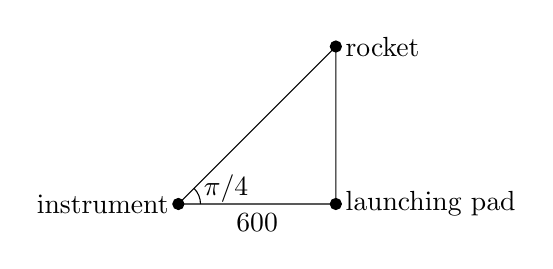
\begin{tikzpicture}
            \coordinate (A) at (2, 2);
            \draw (0, 0) -- node[below]{600} (A |- 0, 0) -- (A) -- (0, 0);
            \draw (8pt, 0) arc[radius=8pt, start angle=0, end angle=45]
            node[right]{$\pi/4$};  
            \filldraw (0, 0) circle(2pt) node[left] {instrument};
            \filldraw (A |- 0, 0) circle(2pt) node[right] {launching pad};
            \filldraw (A) circle (2pt) node[right] {rocket};
          \end{tikzpicture} &&
          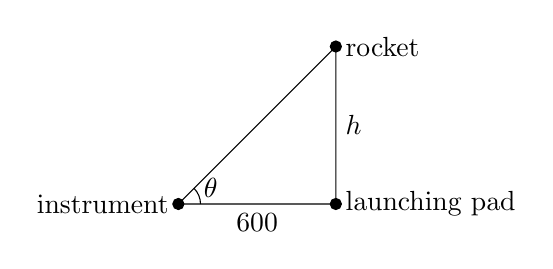
\begin{tikzpicture}
            \coordinate (A) at (2, 2);
            \draw (0, 0) -- node[below]{600} (A |- 0, 0) -- node[right]
            {$h$} (A) -- (0, 0);
            \draw (8pt, 0) arc[radius=8pt, start angle=0, end angle=45]
            node[right]{$\theta$};
            \filldraw (0, 0) circle(2pt) node[left] {instrument};
            \filldraw (A |- 0, 0) circle(2pt) node[right] {launching pad};
            \filldraw (A) circle (2pt) node[right] {rocket};
          \end{tikzpicture}
        \end{tabular}
      \end{center}

      \ideas{Next, we figure out what we know and what we want to know.}

      \highlight{
        \textbf{What we know:} $\frac{d\theta}{dt} = 0.5$ (positive
        because $\theta$ is increasing)

        \textbf{What we want to know:} $\frac{dh}{dt}$
      }

      \ideas{Now, we try to relate variables.  In this case, since the
        rate we know is $\frac{d\bm{\theta}}{dt}$ and the rate we want to
        know is $\frac{d\bm{h}}{dt}$, we try to relate $\theta$ and $h$.}

      \highlight{\textbf{Equation relating our variables:} $\tan \theta =
        \frac{h}{600}$} 

      \ideas{Once we have our relating equation, we differentiate it.  Since
        we are looking for $\frac{dh}{d\bm{t}}$, we should differentiate
        with respect to $t$.}
      \begin{align}
        \frac{d}{dt} \left( \tan \theta \right) &= \frac{d}{dt} \left(
          \frac{h}{600} \right) \nonumber \\
        \sec^2 \theta \frac{d\theta}{dt} &= \frac{1}{600}
        \frac{dh}{dt}
 \\
        \shortintertext{Plug in the snapshot information:} %
        \sec^2 \left( \frac{\pi}{4} \right) \cdot 0.5 &= \frac{1}{600}
        \frac{dh}{dt} \nonumber \\
        \shortintertext{$\cos \left( \frac{\pi}{4} \right) =
          \frac{1}{\sqrt{2}}$, so $\sec \left( \frac{\pi}{4} \right) =
          \sqrt{2}$:} %
        2 \cdot 0.5 &= \frac{1}{600} \frac{dh}{dt}, \nonumber
      \end{align}
      so $\dfrac{dh}{dt} = \boxed{600 \text{ ft/s}}$. 
    \end{solution}

  \item
    \begin{problem}[\stretch{0.5}]
      If the rocket continues climbing at the same vertical speed, does
      the instrument need to speed up, slow down, or continue
      rotating at the same speed to keep tracking the rocket?
    \end{problem}

    \begin{solution}
      This question is asking: if $\frac{dh}{dt}$ remains $600$ ft/s, what
      happens to $\frac{d\theta}{dt}$?  We can use equation (1) to answer
      this: if we plug in $\frac{dh}{dt} = 600$, it says
      \begin{align*}
        \sec^2 \theta \frac{d\theta}{dt} &= 1 \\
        \frac{d\theta}{dt} &= \cos^2 \theta
      \end{align*}
      By common sense, as the rocket continues to rise, $\theta$ must
      increase but remain less than $\frac{\pi}{2}$.  As this happens,
      $\cos^2 \theta$ decreases.  So, as time goes on,
      $\frac{d\theta}{dt}$ remains positive but decreases, so the
      instrument must \fbox{slow down}.
    \end{solution}

  \end{enumerate}

  \pspace{\newpage}

\item 
  Cody has a laser pointer mounted on a
  stand that can be rotated horizontally.  The stand is located 4 meters
  from a wall.  Cody begins with the laser pointer parallel to the wall,
  and he then starts to rotate the laser pointer toward the wall at a
  constant rate of 1/6 radians per second.  (Ignore the length of the
  laser pointer; we'll assume that it is negligible.)

  \begin{enumerate}
  \item
    \begin{problem}[\vfill\vfill]
      When the laser dot on the wall is exactly 5 meters away from the
      laser pointer, how quickly is the light on the wall moving?
    \end{problem}

    \begin{solution}
      This is a related rates problem because we are given information
      about a rate, and we want to find another rate.

      \ideas{As usual, let's start by drawing two pictures, a generic
        picture that applies at any time, and a ``snapshot'' showing the
        situation at the time we care about.  We'll also label some
        variables in the generic picture.}

      Imagine that we are looking down from above. The direction
      the laser pointer is rotating doesn't affect the speed of the
      dot, so let's say it
      is rotating clockwise. Then, we have a picture like this:
      \begin{center}
        \begin{tabular}{ccc}
          \emph{Snapshot} & \hspace{0.25in} & \emph{Generic} \\
          \begin{tikzpicture}
            \coordinate (laser) at (0, -2); %
            \coordinate (dot) at (1.5, 0); %
            \coordinate (A) at (0,-2);
            \coordinate (B) at (0,0);
            \coordinate (C) at (2,0);
            \draw (-0.5,0) -- (2,0) node[right]{wall}; %
            \draw[dashed] (laser) -- node[left] {$4$}
            (laser |- dot); 
            \draw[red] (laser) -- node[anchor=north west]
            {$5$}
            (dot);
            \filldraw (laser) circle(1.5pt) node[below]{laser pointer};
            \filldraw[red] (dot) circle(1.5pt);
            \pic [draw,angle radius=5] {right angle=A--B--C};
          \end{tikzpicture}
          &&
          \begin{tikzpicture}
            \coordinate (laser) at (0, -2); %
            \coordinate (dot) at (2, 0); %
            \coordinate (A) at (0,-2);
            \coordinate (B) at (0,0);
            \coordinate (C) at (2,0);
            \draw (-0.5,0) -- (2.5,0)
            node[right]{wall}; %
            \draw[dashed] (laser) -- node[left] {$4$} 
            (laser |- dot); %
            \draw[red] (laser) -- (dot);
            \draw[decorate, decoration={brace}] ($(laser |- dot) + (0,
            2pt)$) -- node[above, yshift=2pt]{$x$} ($(dot) + (0,
            2pt)$); %
            \filldraw (laser) circle(1.5pt) node[below]{laser pointer}; %
            \filldraw[red] (dot) circle(1.5pt); %
            \pic [draw, <-, angle radius=10, angle eccentricity = 2,
            "$\theta$"] {angle=dot--laser--B};
            \draw[blue, ->] ($(dot) + (2pt, -4pt)$) -- ++(12pt, 0); %
            \pic [draw,angle radius=5] {right angle=A--B--C};
          \end{tikzpicture} 
        \end{tabular}
      \end{center}      
      As shown in the picture, we've let $\theta$ be the angle measured
      clockwise from the vertical line to the laser beam.  (If the laser
      is pointing to the left of the vertical line, then $\theta$ will be
      negative.)  Let $x$ be the distance shown in the diagram; again, if
      the laser is pointing to the left of the vertical line, then $x$
      will be negative. Notice that both $\theta$ and $x$ depend on time $t$.
      
      Also notice that there are two possibilities for
      the dot being \qty{5}{m} away from the laser pointer, one
      to the left of the vertical line and one to the right. Because
      of the symmetry in this case, we
      can use either of them and will get the same answer. (You can
      verify this for yourself.)

      \ideas{Next, we figure out what we know and what we want to know.}

      \highlight{        
        \textbf{What we know:} $\frac{d \theta}{dt} = \frac{1}{6}$ radians
        per second

        \textbf{What we want to know:} $\frac{dx}{dt}$ when the 
        dot is \qty{5}{\meter} away from the laser pointer
      }

      \ideas{Now, we try to relate variables.  In this case, since the
        rate we know is $\frac{d\bm{\theta}}{dt}$ and the rate we want to
        know is $\frac{d\bm{x}}{dt}$, we try to relate $\theta$ and $x$.}
      From our generic picture,

      \highlight{\textbf{Equation relating our variables:} $\tan \theta =
        \frac{x}{4}$}

      \ideas{Once we have our relating equation, we differentiate it.
        Since we are looking for $\frac{dx}{d\bm{t}}$, we should
        differentiate with respect to $t$.}
      \begin{align}
        \frac{d}{dt} (\tan \theta) &= \frac{d}{dt} \left( \frac{x}{4}
        \right) \nonumber \\
        \sec^2 \theta \cdot \frac{d\theta}{dt} &= \frac{1}{4} \cdot
        \frac{dx}{dt}
      \end{align}
      Now, we plug in the snapshot information; at the moment we're
      interested in, $\cos \theta = \frac{4}{5}$, so $\sec \theta =
      \frac{5}{4}$.  Plugging this into
      (1),
      \[ \left( \frac{5}{4} \right)^2 \cdot \frac{1}{6} = \frac{1}{4}
      \cdot \frac{dx}{dt}.\] Solving, $\displaystyle \frac{dx}{dt} =
      \boxed{\frac{25}{24} \text{ m/s.}}$
    \end{solution}

  \item

    \begin{problem}[\vfill\newpage]
      At what point along the wall is the laser dot moving most slowly?
      (You may assume that the wall is infinitely long.)
    \end{problem}

    \begin{solution}
      Now, we're trying to minimize the speed of the laser dot.  The speed
      is $\left| \frac{dx}{dt} \right|$; since we're envisioning the laser
      pointer always moving clockwise, $x$ is always increasing, so
      $\frac{dx}{dt}$ is always positive.  Therefore, we don't need the
      absolute value, which simplifies our goal:

      \highlight{\textbf{Goal:} Minimize $\frac{dx}{dt}$}

      We already found a nice formula for $\frac{dx}{dt}$, equation 
      (1); if we rewrite
      that, we get
      \[ \frac{dx}{dt} = 4 \sec^2 \theta \frac{d\theta}{dt}.\]
      We also know that $\frac{d\theta}{dt}$ is always $\frac{1}{6}$
      radians per second, so we can simplify the above equation to say

      \highlight{\textbf{Formula for thing we're trying to minimize:}
        $\displaystyle \frac{dx}{dt} = 4 \sec^2 \theta \cdot \frac{1}{6} =
        \frac{2}{3} \sec^2 \theta$}

      Thus, we are really trying to minimize $\frac{2}{3} \sec^2 \theta$.
      Before we can do this, we need to figure out the domain of $\theta$.
      In order to have the laser pointer pointing at the wall, $\theta$
      must be in $\left( - \frac{\pi}{2}, \frac{\pi}{2} \right)$.

      We could certainly minimize $\displaystyle \frac{2}{3} \sec^2
      \theta$ on $\displaystyle \left( - \frac{\pi}{2}, \frac{\pi}{2}
      \right)$ by finding critical points and testing them, but there is a
      much easier strategy!  We can rewrite $\frac{2}{3} \sec^2 \theta$ as
      $\frac{2}{3 \cos^2 \theta}$.  In order to make this as small as
      possible, we want to make $\cos^2 \theta$ as \textbf{big} as
      possible.  Using what we know about the cosine function, the biggest
      $\cos^2 \theta$ can be is 1, and this happens when $\cos \theta =
      \pm 1$.  On the interval $\left( - \frac{\pi}{2}, \frac{\pi}{2}
      \right)$, the only time $\cos \theta = \pm 1$ is when $\theta = 0$.
      So, the laser dot is moving most slowly when $\theta = 0$, which is
      \fbox{when the laser is pointing directly at the wall}.
    \end{solution}

  \end{enumerate}


\item
\begin{problem}[\vfill]
  What angle of launch will propel an object (a baseball, football,
  or cannonball) farthest horizontally? This question is important
  to engineers and sportsmen alike. If we consider only the force of
  gravity, then if we launch an object from ground level at an angle
  $\theta$ with an initial velocity of $v_0$, the horizontal
  distance it will travel is given by
  \[R(\theta)=\frac{2(v_0)^2\cos\theta\sin\theta}{g},\]
  where $g$ is the acceleration due to gravity. Find $\theta$ such
  that $R(\theta)$ is maximum. 
\end{problem}

\begin{solution}
Using the double angle identity $\sin(2\theta)=2\sin\theta\cos\theta$,
$R(\theta)$ can be rewritten as 
\[R(\theta)=\frac{(v_0)^2\sin(2\theta)}{g} \text{\quad or \quad} 
\frac{(v_0)^2}{g} \sin(2\theta),\]
where $g$ and $v_0$ are constants. The domain is 
$0\leq\theta\leq\pi/2$.

The simplest approach would be to do this optimization entirely without calculus. Since $R(\theta)$ is equal to some constant times 
$\sin(2\theta)$, we can maximize $R(\theta)$ by by finding the value 
of $\theta$ that maximizes $\sin(2\theta)$. On our domain, 
$\sin(2\theta)=1$ when $\theta=\pi/4$. The optimal launch angle is 
\ang{45}.

Another approach to this problem is to find the critical points and use the Closed Interval Method. The
critical points of $R(\theta)$ are the endpoints $\theta=0$ and 
$\theta=\pi/2$, and the values of 
$\theta$ such that $\frac{dR}{d\theta}=0$.
\begin{align*}
\frac{dR}{d\theta} &= \frac{(v_0)^2}{g} (2\cos(2\theta)) \\
\shortintertext{Setting $\frac{dR}{d\theta}$ equal to 0 gives}
0 &= 2\frac{(v_0)^2}{g}\cos(2\theta) \\
0 &= \cos(2\theta)
\end{align*}

In order to solve this equation, we can first think about the inputs
that make the cosine function equal to zero. This happens at 
$\cos(\pi/2)$, $\cos(3\pi/2$), $\cos(5\pi/2)$, and any angle 
corresponding to the one of the two points on the unit circle where 
$x=0$. (These are the odd multiples of $\pi/2$.) 

Since we have
the equation $\cos(2\theta)=0$, we need
to determine the values of $\theta$ for which $2\theta$, the input
to the cosine function, is one of
the angles we just mentioned. The only such value on our domain is 
$\theta = \pi/4$. This is a candidate for the maximum.

To identify the absolute maximum value, we can
compare the value of $R(\theta)$ at each of our candidate critical
points.
\begin{align*}
R(0) &= 0, \\
R(\pi/4) &= \frac{(v_0)^2}{g}, \\
R(\pi/2) &= 0.
\end{align*}

Therefore $R(\theta)$ is maximized when $\theta = \pi/4$.

% We can show it is actually the maximum by looking at $R''(\theta)$ or
% $\diff[2]{R}{\theta}$.
% \begin{multicols}{2}

% \begin{align*}
% R''(\theta) &= \frac{2(v_0)^2}{g}\,\diff*{2\cos(2\theta)}{x} \\
% &= \frac{2(v_0)^2}{g} (-2\sin(2\theta)) \\
% &= \frac{-4(v_0)^2}{g} \sin(2\theta)
% \end{align*}

% \columnbreak

% \begin{align*}
% R''(\pi/4) &= \frac{-4(v_0)^2}{g} \sin(\pi/2) \\
% &= \frac{-4(v_0)^2}{g} \\
% &< 0 \phantom{\frac{1}{x}}
% \end{align*}

% \end{multicols}
% $R''(\pi/4)<0$, so the graph of $R(\theta)$ is concave down at $\theta = \pi/4$
% and $R(\theta)$ has a maximum at $\theta=\pi/4$. Therefore an angle of
% $\frac{\pi}{4}$ radians, or $\ang{45}$, is the angle that will give the greatest
% horizontal distance.
\end{solution}

\end{enumerate}
\end{document}